\documentclass{article}

\def \lastexercisenumber{18}

% Hier befinden sich Pakete, die wir beinahe immer benutzen ...

\usepackage[utf8]{inputenc}

% Sprach-Paket:
\usepackage[ngerman]{babel}

% damit's nicht so, wie beim Grill aussieht:
\usepackage{fullpage}

% Mathematik:
\usepackage{amsmath, amssymb, amsfonts, amsthm}
\usepackage{bbm}
\usepackage{mathtools, mathdots}

% Makros mit mehereren Default-Argumenten:
\usepackage{twoopt}

% Anführungszeichen (Makro \Quote{}):
\usepackage{babel}

% if's für Makros:
\usepackage{xifthen}
\usepackage{etoolbox}

% tikz ist kein Zeichenprogramm (doch!):
\usepackage{tikz}

% bessere Aufzählungen:
\usepackage{enumitem}

% (bessere) Umgebung für Bilder:
\usepackage{graphicx, subfig, float}

% Umgebung für Code:
\usepackage{listings}

% Farben:
\usepackage{xcolor}

% Umgebung für "plain text":
\usepackage{verbatim}

% Umgebung für mehrerer Spalten:
\usepackage{multicol}

% "nette" Brüche
\usepackage{nicefrac}

% Spaltentypen verschiedener Dicke
\usepackage{tabularx}
\usepackage{makecell}

% Für Vektoren
\usepackage{esvect}

% (Web-)Links
\usepackage{hyperref}

% Zitieren & Literatur-Verzeichnis
\usepackage[style = authoryear]{biblatex}
\usepackage{csquotes}

% so ähnlich wie mathbb
%\usepackage{mathds}

% Keine Ahnung, was das macht ...
\usepackage{booktabs}
\usepackage{ngerman}
\usepackage{placeins}

% special letters:

\newcommand{\N}{\mathbb{N}}
\newcommand{\Z}{\mathbb{Z}}
\newcommand{\Q}{\mathbb{Q}}
\newcommand{\R}{\mathbb{R}}
\newcommand{\C}{\mathbb{C}}
\newcommand{\K}{\mathbb{K}}
\newcommand{\T}{\mathbb{T}}
\newcommand{\E}{\mathbb{E}}
\newcommand{\V}{\mathbb{V}}
\renewcommand{\S}{\mathbb{S}}
\renewcommand{\P}{\mathbb{P}}
\newcommand{\1}{\mathbbm{1}}

% quantors:

\newcommand{\Forall}{\forall \,}
\newcommand{\Exists}{\exists \,}
\newcommand{\ExistsOnlyOne}{\exists! \,}
\newcommand{\nExists}{\nexists \,}
\newcommand{\ForAlmostAll}{\forall^\infty \,}

% MISC symbols:

\newcommand{\landau}{{\scriptstyle \mathcal{O}}}
\newcommand{\Landau}{\mathcal{O}}


\newcommand{\eps}{\mathrm{eps}}

% graphics in a box:

\newcommandtwoopt
{\includegraphicsboxed}[3][][]
{
  \begin{figure}[!h]
    \begin{boxedin}
      \ifthenelse{\isempty{#1}}
      {
        \begin{center}
          \includegraphics[width = 0.75 \textwidth]{#3}
          \label{fig:#2}
        \end{center}
      }{
        \begin{center}
          \includegraphics[width = 0.75 \textwidth]{#3}
          \caption{#1}
          \label{fig:#2}
        \end{center}
      }
    \end{boxedin}
  \end{figure}
}

% braces:

\newcommand{\pbraces}[1]{{\left  ( #1 \right  )}}
\newcommand{\bbraces}[1]{{\left  [ #1 \right  ]}}
\newcommand{\Bbraces}[1]{{\left \{ #1 \right \}}}
\newcommand{\vbraces}[1]{{\left  | #1 \right  |}}
\newcommand{\Vbraces}[1]{{\left \| #1 \right \|}}
\newcommand{\abraces}[1]{{\left \langle #1 \right \rangle}}
\newcommand{\round}[1]{\bbraces{#1}}

\newcommand
{\floorbraces}[1]
{{\left \lfloor #1 \right \rfloor}}

\newcommand
{\ceilbraces} [1]
{{\left \lceil  #1 \right \rceil }}

% special functions:

\newcommand{\norm}  [2][]{\Vbraces{#2}_{#1}}
\newcommand{\diam}  [2][]{\mathrm{diam}_{#1} \: #2}
\newcommand{\diag}  [1]{\mathrm{diag} \: #1}
\newcommand{\dist}  [1]{\mathrm{dist} \: #1}
\newcommand{\mean}  [1]{\mathrm{mean} \: #1}
\newcommand{\erf}   [1]{\mathrm{erf} \: #1}
\newcommand{\id}    [1]{\mathrm{id} \: #1}
\newcommand{\sgn}   [1]{\mathrm{sgn} \: #1}
\newcommand{\supp}  [1]{\mathrm{supp} \: #1}
\newcommand{\arsinh}[1]{\mathrm{arsinh} \: #1}
\newcommand{\arcosh}[1]{\mathrm{arcosh} \: #1}
\newcommand{\artanh}[1]{\mathrm{artanh} \: #1}
\newcommand{\card}  [1]{\mathrm{card} \: #1}
\newcommand{\Span}  [1]{\mathrm{span} \: #1}
\newcommand{\Aut}   [1]{\mathrm{Aut} \: #1}
\newcommand{\End}   [1]{\mathrm{End} \: #1}
\newcommand{\ggT}   [1]{\mathrm{ggT} \: #1}
\newcommand{\kgV}   [1]{\mathrm{kgV} \: #1}
\newcommand{\ord}   [1]{\mathrm{ord} \: #1}
\newcommand{\grad}  [1]{\mathrm{grad} \: #1}
\newcommand{\ran}   [1]{\mathrm{ran} \: #1}
\newcommand{\graph} [1]{\mathrm{graph} \: #1}
\newcommand{\Inv}   [1]{\mathrm{Inv} \: #1}
\newcommand{\pv}    [1]{\mathrm{pv} \: #1}
\newcommand{\GL}    [1]{\mathrm{GL} \: #1}
\newcommand{\Mod}{\mathrm{Mod} \:}
\newcommand{\Th}{\mathrm{Th} \:}
\newcommand{\Char}{\mathrm{char}}
\newcommand{\At}{\mathrm{At}}
\newcommand{\Ob}{\mathrm{Ob}}
\newcommand{\Hom}{\mathrm{Hom}}
\newcommand{\orthogonal}[3][]{#2 ~\bot_{#1}~ #3}
\newcommand{\Rang}{\mathrm{Rang}}
\newcommand{\NIL}{\mathrm{NIL}}
\newcommand{\Res}{\mathrm{Res}}
\newcommand{\lxor}{\dot \lor}
\newcommand{\Div}{\mathrm{div} \:}
\newcommand{\meas}{\mathrm{meas} \:}

% fractions:

\newcommand{\Frac}[2]{\frac{1}{#1} \pbraces{#2}}
\newcommand{\nfrac}[2]{\nicefrac{#1}{#2}}

% derivatives & integrals:

\newcommandtwoopt
{\Int}[4][][]
{\int_{#1}^{#2} #3 ~\mathrm{d} #4}

\newcommandtwoopt
{\derivative}[3][][]
{
  \frac
  {\mathrm{d}^{#1} #2}
  {\mathrm{d} #3^{#1}}
}

\newcommandtwoopt
{\pderivative}[3][][]
{
  \frac
  {\partial^{#1} #2}
  {\partial #3^{#1}}
}

\newcommand
{\primeprime}
{{\prime \prime}}

\newcommand
{\primeprimeprime}
{{\prime \prime \prime}}

% Text:

\newcommand{\Quote}[1]{\glqq #1\grqq{}}
\newcommand{\Text}[1]{{\text{#1}}}
\newcommand{\fastueberall}{\text{f.ü.}}
\newcommand{\fastsicher}{\text{f.s.}}

% -------------------------------- %
% amsthm-stuff:

\theoremstyle{definition}

% numbered theorems
\newtheorem{theorem}{Satz}
\newtheorem{lemma}{Lemma}
\newtheorem{corollary}{Korollar}
\newtheorem{proposition}{Proposition}
\newtheorem{remark}{Bemerkung}
\newtheorem{definition}{Definition}
\newtheorem{example}{Beispiel}

% unnumbered theorems
\newtheorem*{theorem*}{Satz}
\newtheorem*{lemma*}{Lemma}
\newtheorem*{corollary*}{Korollar}
\newtheorem*{proposition*}{Proposition}
\newtheorem*{remark*}{Bemerkung}
\newtheorem*{definition*}{Definition}
\newtheorem*{example*}{Beispiel}

% Please define this stuff in project ("main.tex"):

% \def \lastexercisenumber {...}
% This will be 0 by default

% \setcounter{section}{...}
% This will be 0 by default
% and hence, completely ignored

\ifnum \thesection = 0
{\newtheorem{exercise}{Aufgabe}}
\else
{\newtheorem{exercise}{Aufgabe}[section]}
\fi

\ifdef
{\lastexercisenumber}
{\setcounter{exercise}{\lastexercisenumber}}

\newcommand{\solution}
{
    \renewcommand{\proofname}{Lösung}
    \renewcommand{\qedsymbol}{}
    \proof
}

\renewcommand{\proofname}{Beweis}

% -------------------------------- %
% environment zum einkasteln:

% dickere vertical lines
\newcolumntype
{x}
[1]
{!{\centering\arraybackslash\vrule width #1}}

% environment selbst (the big cheese)
\newenvironment
{boxedin}
{
  \begin{tabular}
  {
    x{1 pt}
    p{\textwidth}
    x{1 pt}
  }
  \Xhline
  {2 \arrayrulewidth}
}
{
  \\
  \Xhline{2 \arrayrulewidth}
  \end{tabular}
}

% -------------------------------- %
% MISC "Ein-Deutschungen"

\renewcommand
{\figurename}
{Abbildung}

\renewcommand
{\tablename}
{Tabelle}

% -------------------------------- %


\addbibresource{../../../Fundament-LaTeX/references.bib}

\graphicspath{{../../../Fundament-LaTeX/images/}}

\parindent 0pt

\title
{
  Diskrete und Geometrische Algorithmen \\
  \vspace{4pt}
  \normalsize
  \textit{4. Übung am 16.11.2020}
}
\author
{
  Richard Weiss
  \and
  Florian Schager
  \and
  Christian Sallinger
  \and
  Fabian Zehetgruber
  \and
  Paul Winkler
  \and
  Christian Göth
}
\date{}

\begin{document}

\maketitle

% --------------------------------------------------------------------------------

\begin{exercise}

	Lösen Sie die Rekursion $n a_n = (n + 1) a_{n - 1} + 2n$ mit $a_0 = 2$. 

\end{exercise}


\begin{solution}

	Wir dividieren auf beiden Seiten durch $n$ und erhalten die Rekursionsgleichung 
	\begin{align*}
	a_n = \frac{n + 1}{n} a_{n - 1} + 2, \quad a_1 = 2
	\end{align*}
	Um diese auf die Form des Skriptums zu bringen definieren wir $x_n := a_{n + 1}$ und erhalten 
	\begin{align*}
	x_n = \frac{n + 2}{n + 1} x_{n -1} + 2, \quad x_0 = 2
	\end{align*}
	Nun wissen wir aus Satz 4.1, dass 
	\begin{align*}
	x_n = \sum_{i = 0}^n 2 \prod_{j =  i + 1}^n \frac{j + 2}{j + 1}  = 2 \sum_{i = 0}^n \prod_{j =  i + 1}^n \frac{j + 2}{j + 1} = 2 \sum_{i = 0}^n \frac{n + 2}{i + 2} = 2 (n + 2) \sum_{i=2}^{n+2} \frac{1}{i} 
	\end{align*}
	Eine Lösung der Rekursionsgleichung ist. Mit Induktion erkennen wir
	\begin{align*}
	\prod_{j=i+1}^i = 1 = \frac{i + 1}{i +1}, \quad \prod_{j = i+1}^{n + 1} \frac{j + 2}{j + 1} = \frac{n + 3}{n + 2} \frac{n + 2}{i + 1} = \frac{(n + 1) + 2}{i + 1}
	\end{align*}
	und 
	\begin{align*}
	\sum_{i = 2}^2 \frac{1}{i} = \frac{1}{2}, \quad \sum_{i = 2}^{n + 3} \frac{1}{i} = ?
	\end{align*}
\end{solution}

% --------------------------------------------------------------------------------

% --------------------------------------------------------------------------------

\begin{exercise}

\phantom{}

\begin{enumerate}[label = \textbf{\alph*)}]

  \item Es sei $\Omega = (0,1), t >0, f \in L^2(\Omega)$, und $X := H^1_D(\Omega) \times H^1_D(\Omega)$ mit $H^1_D(\Omega) := \Bbraces{u \in H^1(\Omega) | u(0) = 0}$.
  Das Problem des Timoshenko Balkens lautet:
  Gesucht ist $(w, \beta) \in X$ sodass für alle $(v, \delta) \in X$

  \begin{align}
    \Int[\Omega]{\beta^\prime \delta^\prime}{x}
    +
    \frac{1}{t^2} \Int[\Omega]{(w^\prime - \beta)(v^\prime - \delta)}{x}
    =
    \Int[\Omega]{f v}{x}.
  \end{align}

  Zeigen Sie, dass das Problem eindeutig lösbar ist. Wie verhält sich die Konstante in Cea's Lemma wenn $t \to 0$?
  \textit{Hinweis}:
  Verwenden Sie wie in Aufgabe 19 die Young Ungleichung für den gemischten Term sowie die Friedrich Ungleichung.

  \item Sei nun $\Omega \subset \R^2$ und $X := H^1_D(\Omega) \times [H^1_D(\Omega)]^2$.
  Betrachten Sie die Reissner-Mindlin Platte als zweidimiensionale Erweiterung des Timoshenko Balkens beschrieben durch das Problem:
  Gesucht ist $(w, \beta) \in X$ sodass für alle $(v, \delta) \in X$

  \begin{align}
    \Int[\Omega]{\epsilon(\beta):\epsilon(\delta)}{x}
    +
    \frac{1}{t^2} \Int[\Omega]{(\nabla w - \beta) \cdot (\nabla v - \delta)}{x}
    =
    \Int[\Omega]{f v}{x},
  \end{align}

  wobei $\epsilon(\beta) := 0.5 (\nabla \beta + (\nabla \beta)^\top)$ der symmetrische Gradient ist.
  Untersuchen Sie mit dem zur Verfügung gestellten Jupyter-File das Konvergenzverhalten für lineare Elemente bei verschiedenen Dickenparametern, $t \in \Bbraces{1, 0.1, 0.01, 0.001}$.
  Was beobachten Sie?
  Wie ändert sich das Verhalten für quadratisch finite Elemente?

\end{enumerate}

\end{exercise}

% --------------------------------------------------------------------------------

\begin{solution}

\phantom{}

\begin{enumerate}[label = \textbf{\alph*)}]

  \item Wir wollen wieder Exercise 7 (Lemma of Lax-Milgram) anwenden, diesmal mit

  \begin{align*}
    a
    \pbraces
    {
      \begin{pmatrix}
        w \\ \beta
      \end{pmatrix},
      \begin{pmatrix}
        v \\ \xi
      \end{pmatrix}
    }
    :=
    \Int[\Omega]{\beta^\prime \delta^\prime}{x}
    +
    \frac{1}{t^2} \Int[\Omega]{(w^\prime - \beta)(v^\prime - \delta)}{x},
    \quad
    F
    \begin{pmatrix}
      v \\ \delta
    \end{pmatrix}
    :=
    \Int[\Omega]{f v}{x}.
  \end{align*}

  \begin{enumerate}[label = \arabic*.]

    \item Schritt (Stetigkeit von $a$):
    
    Auf dem $\R^2$ sind die Normen $\norm[1]{\cdot}$ und $\norm[2]{\cdot}$ äquivalent.
    Wir erhalten also eine Konstante $C > 0$, sodass $\norm[1]{\cdot} \leq C \norm[2]{\cdot}$.

    \begin{align*}
      \norm[1]{\cdot}
      \sim
      \norm[2]{\cdot}
      ~\text{auf $\R^2$}~
      \implies
      \Exists C > 0:
      \norm[1]{\cdot}
      \leq
      C
      \norm[2]{\cdot}
    \end{align*}

    Vorausschauend auf das Lemma 1.6 (Céa), definieren wir noch die Konstante

    \begin{align*}
      \beta_t
      :=
      2 \max \Bbraces{1, \frac{1}{t^2}} C.
    \end{align*}

    \begin{align*}
      a
      \pbraces
      {
        \begin{pmatrix}
          w \\ \beta
        \end{pmatrix},
        \begin{pmatrix}
          v \\ \xi
        \end{pmatrix}
      }
      & =
      \Int[\Omega]{\beta^\prime \delta^\prime}{x}
      +
      \frac{1}{t^2} \Int[\Omega]{(w^\prime - \beta)(v^\prime - \delta)}{x} \\
      & \stackrel
      {
        \mathrm{CSB}
      }{\leq}
      \norm[L^2(\Omega)]{\beta^\prime}
      \norm[L^2(\Omega)]{\delta^\prime}
      +
      \frac{1}{t^2}
      \norm[L^2(\Omega)]{w^\prime - \beta}
      \norm[L^2(\Omega)]{v^\prime - \delta} \\
      & \leq
      \norm[L^2(\Omega)]{\beta^\prime}
      \norm[L^2(\Omega)]{\delta^\prime}
      +
      \frac{1}{t^2}
      \pbraces
      {
        \norm[L^2(\Omega)]{w^\prime}
        \norm[L^2(\Omega)]{\beta}
      }
      \pbraces
      {
        \norm[L^2(\Omega)]{v^\prime}
        \norm[L^2(\Omega)]{\delta}
      } \\
      & \leq
      2 \max \Bbraces{1, \frac{1}{t^2}}
      \pbraces
      {
        \norm[L^2(\Omega)]{w^\prime}
        \norm[L^2(\Omega)]{\beta}
      }
      \pbraces
      {
        \norm[L^2(\Omega)]{v^\prime}
        \norm[L^2(\Omega)]{\delta}
      } \\
      & = \cdots \leq
      2 \max \Bbraces{1, \frac{1}{t^2}} C
      \pbraces
      {
        \norm[L^2(\Omega)]{w^\prime}^2
        \norm[L^2(\Omega)]{\beta}^2
      }^{1/2}
      \pbraces
      {
        \norm[L^2(\Omega)]{v^\prime}^2
        \norm[L^2(\Omega)]{\delta}^2
      }^{1/2} \\
      & =
      \beta_t
      \norm[X]
      {
        \begin{pmatrix}
          w \\ \beta
        \end{pmatrix}
      }
      \norm[X]
      {
        \begin{pmatrix}
          v \\ \delta
        \end{pmatrix}
      }
    \end{align*}

    \item Schritt (Elliptizität von $a$):
    
    \begin{enumerate}[label = \arabic*.]

      \item Hilfs-Ungleichung (Friedrich):

      \begin{center}
        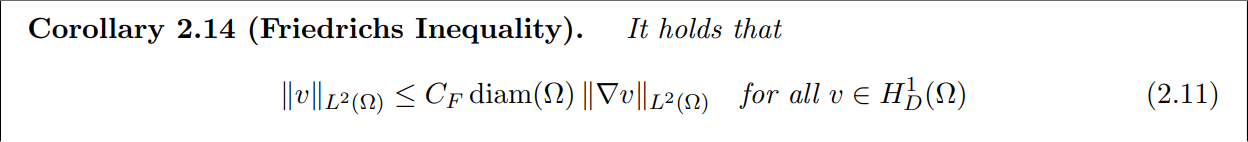
\includegraphics[width = 0.75 \textwidth]{NumPDEs/NumPDEs - Corollary 2.14.1 (Friedrichs Inequality).png} \\
        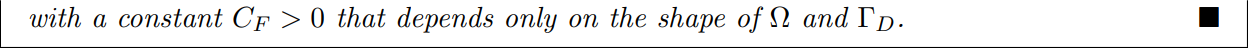
\includegraphics[width = 0.75 \textwidth]{NumPDEs/NumPDEs - Corollary 2.14.2 (Friedrichs Inequality).png}
      \end{center}

      \begin{align*}
        \implies
        \norm[H^1(\Omega)]{v}^2
        =
        \norm[L^2(\Omega)]{v}
        +
        \norm[L^2(\Omega)]{\nabla v}
        \stackrel
        {
          \mathrm{F}
        }{\leq}
        (
          C_F
          \underbrace{\diam \Omega}_1
          +
          1
        )^2
        \norm[L^2(\Omega)]{v^\prime}^2
      \end{align*}

      \item Hilfs-Ungleichung (Young):
      
      Dabei wollen wir $\varepsilon_t$ wie folgt wählen.

      \begin{align*}
        \varepsilon_t
        \in
        \pbraces
        {
          \frac{1}
          {
            1
            +
            \frac{t^2}{(C_F + 1)^2}
          },
          1
        }
        \neq
        \emptyset
      \end{align*}

      Das Intervall ist dabei nicht die leere Menge, weil $t > 0$ und daher

      \begin{align*}
        1 < 1 + \frac{t^2}{(C_F + 1)^2}.
      \end{align*}

    \end{enumerate}

    Vorausschauend auf das Lemma 1.6 (Céa), definieren wir noch die Konstante

    \begin{align*}
      \alpha_t
      :=
      \min
      \Bbraces
      {
        \frac{1}{(C_F + 1)^2}
        +
        \frac{1}{t^2}
        \pbraces
        {
          1 - \frac{1}{\varepsilon_t}
        },
        \frac
        {
          1 - \varepsilon_t
        }{
          t^2 (C_F + 1)^2
        }
      }.
    \end{align*}

    \begin{align*}
      a
      \pbraces
      {
        \begin{pmatrix}
          w \\ \beta
        \end{pmatrix},
        \begin{pmatrix}
          w \\ \beta
        \end{pmatrix}
      }
      & =
      \norm[L^2(\Omega)]{\beta^\prime}^2
      +
      \frac{1}{t^2}
      \Int[\Omega]{\abs{w^\prime - \beta}^2}{x} \\
      & =
      \norm[L^2(\Omega)]{\beta^\prime}^2
      +
      \frac{1}{t^2}
      \pbraces
      {
        \norm[L^2(\Omega)]{w^\prime}^2
        +
        \Int[\Omega]{- 2 w^\prime \beta}{x}
        +
        \norm[L^2(\Omega)]{\beta}^2
      } \\
      & \stackrel
      {
        \mathrm{Y}
      }{\geq}
      \norm[L^2(\Omega)]{\beta^\prime}^2
      +
      \frac{1}{t^2}
      \pbraces
      {
        \norm[L^2(\Omega)]{w^\prime}^2
        +
        \Int[\Omega]{- \varepsilon_t \abs{w^\prime}^2}{x}
        +
        \Int[\Omega]{- \frac{1}{\varepsilon_t} \abs{\beta}^2}{x}
        +
        \norm[L^2(\Omega)]{\beta}^2
      } \\
      & =
      \norm[L^2(\Omega)]{\beta^\prime}^2
      +
      \frac{1}{t^2}
      \pbraces
      {
        (1 - \varepsilon_t)
        \norm[L^2(\Omega)]{w^\prime}^2
        +
        \pbraces
        {
          1 - \frac{1}{\varepsilon_t}
        }
        \norm[L^2(\Omega)]{\beta}^2
      } \\
      & \stackrel
      {
        \mathrm{F}
      }{\geq}
      \frac{1}{(C_F + 1)^2}
      \norm[H^2(\Omega)]{\beta}^2
      +
      \frac{1}{t}
      \pbraces
      {
        \frac{1 - \varepsilon_t}{(C_F + 1)^2}
        \norm[H^1(\Omega)]{w}^2
        +
        \pbraces
        {
          1 - \frac{1}{\varepsilon_t}
        }
        \norm[H^1(\Omega)]{\beta}^2
      } \\
      & =
      \pbraces
      {
        \frac{1}{(C_F + 1)^2}
        +
        \frac{1}{t^2}
        \pbraces
        {
          1 - \frac{1}{\varepsilon_t}
        }
      }
      \norm[H^1(\Omega)]{\beta}^2
      +
      \frac{1 - \varepsilon_t}{t^2 (C_F + 1)^2}
      \norm[H^1(\Omega)]{w}^2 \\
      & \geq
      \min
      \Bbraces
      {
        \frac{1}{(C_F + 1)^2}
        +
        \frac{1}{t^2}
        \pbraces
        {
          1 - \frac{1}{\varepsilon_t}
        },
        \frac
        {
          1 - \varepsilon_t
        }{
          t^2 (C_F + 1)^2
        }
      }
      \pbraces
      {
        \norm[H^1(\Omega)]{w}^2
        +
        \norm[H^1(\Omega)]{\beta}^2
      } \\
      & =
      \alpha_t
      \norm[X]
      {
        \begin{pmatrix}
          w \\ \beta
        \end{pmatrix}
      }^2
    \end{align*}

    \item Schritt (Stetigkeit von $F$):
    
    \begin{align*}
      F
      \begin{pmatrix}
        v \\ \delta
      \end{pmatrix}
      =
      \Int[\Omega]{f v}{x}
      \stackrel
      {
        \mathrm{CSB}
      }{\leq}
      \norm[L^2(\Omega)]{f}
      \norm[L^2(\Omega)]{v}
      \leq
      \norm[L^2(\Omega)]{f}
      \norm[X]
      {
        \begin{pmatrix}
          v \\ \delta
        \end{pmatrix}
      }
    \end{align*}

  \end{enumerate}

  \includegraphicsunboxed{NumPDEs/NumPDEs - Lemma 1.6 (Céa).png}

  Der Quotient in Lemma 1.6 (Céa) divergiert.

  \begin{align*}
    \beta_t
    & =
    2 \max \Bbraces{1, \frac{1}{t^2}} C
    \xrightarrow{t \to 0}
    \infty, \\
    \alpha_t
    & =
    \min
    \Bbraces
    {
      \frac{1}{(C_F + 1)^2}
      +
      \frac{1}{t^2}
      \pbraces
      {
        1 - \frac{1}{\varepsilon_t}
      },
      \frac
      {
        1 - \varepsilon_t
      }{
        t^2 (C_F + 1)^2
      }
    }
    \leq
    \frac
    {
      1 - \varepsilon_t
    }{
      t^2 (C_F + 1)^2
    }
    \leq
    \frac
    {
      1
      -
      \frac{1}
      {
        1
        +
        \frac{t^2}{(C_F + 1)^2}
      }
    }{
      t^2 (C_F + 1)^2
    } \\
    & =
    \frac
    {
      1 + \frac{t^2}{(C_f + 1)^2} - 1
    }{
      \pbraces
      {
        1 + \frac{t^2}{(C_F + 1)^2}
      }
      t^2 (C_F + 1)^2
    }
    =
    \frac{1}
    {
      (C_F + 1)^2
      \pbraces
      {
        (C_F + 1)^2 + t^2
      }
    }
    \xrightarrow{t \to 0}
    \frac{1}{(C_F + 1)^4} \\
    \implies
    \frac{\beta_t}{\alpha_t}
    & \xrightarrow{t \to 0}
    \infty
  \end{align*}

  Die Fehlerschranke (d.h. die rechte Seite von (1.20)) kann also beliebig groß werden.
  Somit können wir Lemma 1.6 (Céa) nicht anwenden, um den FEM-Fehler sinnvoll abzuschätzen.

\end{enumerate}

\end{solution}

% --------------------------------------------------------------------------------


\printbibliography

\end{document}
